\chapter{Automatic Code Generation for RNA}
\label{cap:code_gen}

In this chapter, we present a mechanism for automatic code generation for the RNA Framework. This enables network operators to deploy the framework without having the experience and knowledge to develop software for Zeek or programmable forwarding devices (P4).

The code generation mechanism uses two sets of inputs: the scripts, whose events should be offloaded; a pool of \ProtocolTemplates{} and \Offloader{} Templates. The previously mentioned concepts, the \ProtocolTemplates{} and the \Offloaders{} are used as sources of templates and resources, in order to implement the software required to offload the events subscribed by the desired scripts. We also propose the generation of a unique Zeek Plugin, which will automatically deploy the P4 code when initiated, instead of having two separate deployable components.


% ==============================================================================
%                               OVERVIEW
% ==============================================================================


\section{Overview}
\label{sec:code_gen:overview}

This section presents an overview of the RNA Code Generation Mechanism, starting with its inputs and expected output, which is illustrated in Figure \ref{fig:code_gen_black_box}. The main input for the mechanism is the set of scripts, whose monitoring the network operator is interested in. These scripts need to be provided in their entirety, so we can identify the events to which they subscribe.

\begin{figure}[htb]
    \caption{RNA - Code Generation Mechanism}
    \begin{center}
        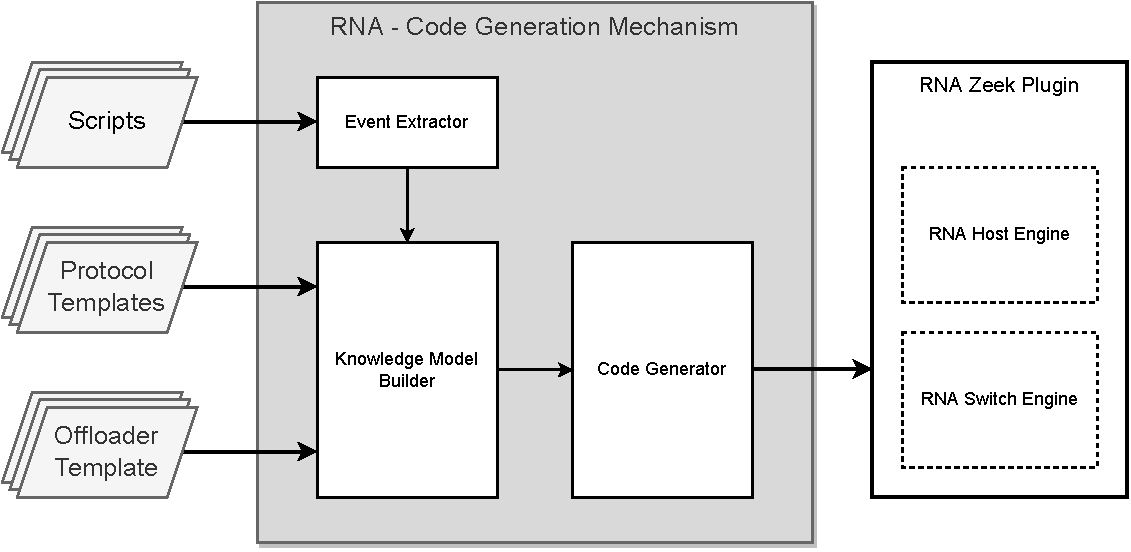
\includegraphics[width=0.98\textwidth]{images/code_gen_mechanism.pdf}
    \end{center}
    \label{fig:code_gen_black_box}
    \legend{Source: the author}
\end{figure}

The second set of inputs is what we call \textit{templates}, which can be either  \ProtocolTemplates{} or \Offloader{} Templates. They are a pool of known implementations of protocols and events that can be used to offload scripts. A template being present in this pool does not mean it will be included in the final output, but it means it is available in case its implementation is needed by a script.

The desired output of our mechanism is a single Zeek Plugin following the structure previously presented in Section \ref{sec:rna:overview} and illustrated in Figure \ref{fig:arch_low_level}. This Zeek Plugin when executed should: configure the switch, creating a mirroring session for the Zeek monitoring system, deploying the P4 code; and configure Zeek, registering all Translators in Zeek's Event Engine, and registering the RNA Event Handler. This eliminates the need for the operator to coordinate the deployment of two separate systems, the RNA Host Engine, and the RNA Switch Engine.

To be able to execute this task, the first objective of the code generation process is to analyze all the provided Zeek scripts and identify which are the observed events in every script. Once this pool of events is known, we select \Offloaders{} (from the templates pool) that are capable of offloading those events. This step is finished and succeeds if we find at least one \Offloader{} for every event.

After all events and \Offloaders{} have been selected, the mechanism must ensure all templates for the protocols required by these \Offloaders{} are available. The \ProtocolTemplates{} are required so the \Offloaders{} can interpret the desired headers. After all this knowledge model is complete, the mechanism generates all required source files.

Some of the resulting code that is present in the final Zeek Plugin is extracted and merged from the templates, and not completely generated by our mechanism. It is not yet possible to fully generate all offloader code, because the process of converting C++ or P4 code from one to another is very complicated and is out of the scope of this project.


% 
% Pode revisar até aqui :)
% 

% ==============================================================================
%                            Detailed Mechanism Design
% ==============================================================================

\section{Detailed Mechanism Design}
\label{sec:code_gen_impl}

The operation of our RNA Code Generation Mechanism can be classified into three different stages. The first stage identifies the events that our input scripts subscribe to. The second stage is building our knowledge model, which receives as inputs all \ProtocolTemplates{}, \Offloaders{}, and events of interest, which the network operator requested to be offloaded. We call this knowledge model \textit{ProtocolGraph}. The last stage is the actual code merge and generation process using this structured and validated knowledge model from the previous step. We start explaining the first stage of our mechanism, the extracting the subscribed events from the Zeek Scripts.

\subsection{Event Extraction}

To identify which events a Zeek Script subscribes to, we first need to parse the script as a whole. The mechanism does it using Zeek's provided grammatical definition. After parsing all the scripts, we search the Abstract Syntax Tree for event handlers, returning their event identifiers.

In this stage, the most important important information to be forwarded to the next step is the identifiers of the events we want to offload. Those will indicate the requirements of our deployment. The name of the scripts are also passed to the knowledge model as a logging and debugging asset, but are no longer essential for the final functionality.

\subsection{Knowledge Model}

The core logic behind the implementation of our RNA Code Generation Mechanism relies on a structure we call \textit{ProtocolGraph}. This is a graph structure that stores all protocols required for our events of interest. The \Offloaders{} are linked to their final protocol layer in the graph, generating in the end a structure as presented in Figure \ref{fig:protocol_graph}. This structure is a graph, with a node we assign as root, in most cases, the \textsc{Ethernet} protocol. The other protocols are linked to their respective parents. The Offloaders are linked to the protocol they analyze, which does not need to be a leaf protocol.

\begin{figure}[htb]
    \caption{Knowledge Model - Protocol Graph}
    \begin{center}
        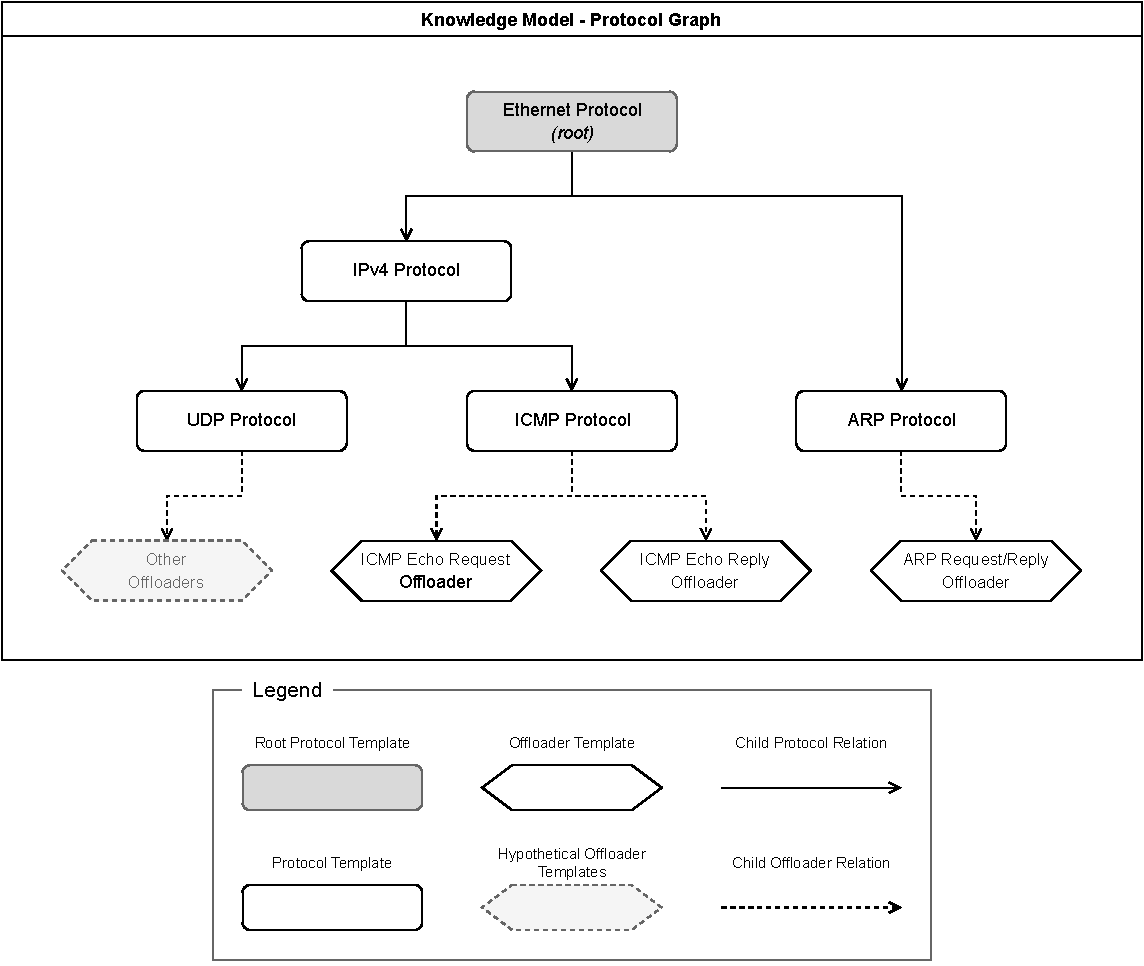
\includegraphics[width=0.98\textwidth]{images/icmp_ex_protocol_graph.pdf}  
    \end{center}
    \label{fig:protocol_graph}
    \legend{Source: the author}
\end{figure}

The algorithm to generate and validate the \textit{ProtocolGraph} is outlined in Algorithm \ref{alg:build_graph}. The pseudo-code will be used to describe and guide the explanation of our algorithm and we will refer to the lines according to their respective roles.

\begin{algorithm}[htb]
    \caption{Knowledge Model Build Algorithm}
    \label{alg:build_graph}
    \SetKwInput{Input}{Input}
    \SetKwInput{Output}{Output}
    
    \Input{$templates$, $events$, $forced\_of\!floaders$}
    \Output{$graph$}
    
    \vspace{1em}

    \Call{ValidateComponentList}{$templates$}

    \vspace{1em}

    $protocols \gets$ FilterListByType($templates$, $ProtocolTemplate$) \\
    $of\!floaders \gets$ \Call{FilterListByType}{$templates$, $Of\!floaderTemplate$} \\
    
    \vspace{1em}
    
    $of\!floaders \gets$ \Call{ReqOffloaders}{$of\!floaders$, $events$, $forced\_of\!floaders$} \\

    \vspace{1em}

    \If{$of\!floaders$ is empty} {
        \textbf{raise} \textit{exception} \Comment{nothing to be offloaded}\\
    }

    \vspace{1em}

    $root \gets$ \Call{FindRootProtocol}{$protocols$} \\
    $graph \gets$ \Call{LinkGraph}{$root$, $protocols$} \\

    \vspace{1em}

    \If{\Call{HasCycles}{$graph$}} {
        \textbf{raise} \textit{exception} \Comment{protocol graph has cycles}\\
    }
    
    \vspace{1em}
    
    $protocols \gets$ \Call{RemoveUnreachableProtocols}{$graph$, $protocols$} \\
    \Call{AttachOffloaders}{$graph, of\!floaders$} \\
    
    \vspace{1em}

    \Call{TrimUnusedProtocols}{$graph$} \\
    
    \vspace{1em}
            
    \Call{SetProtocolDepths}{$graph$} \\
    \Call{SortProtocols}{$graph$} \\
    \Call{SortOffloaders}{$graph$} \\
    \Call{SetOffloadersUids}{$graph$} \\
    
    \vspace{1em}
            
    \textbf{return} $graph$ \Comment{successfull graph generation} \\
\end{algorithm}


\subsubsection*{Template loading and filtering}
% Lines 1 - 6

As the mechanism is executed, the first step is to load all templates and validate their versions, files and requirements. All the templates are loaded and stored in a list, even if they are not used later in the final model. After the templates are loaded, we separate them between Protocol Templates and Offloader Templates. This happens on lines 1 to 3 in Algorithm \ref{alg:build_graph}.

After all offloader templates are validated, we select what offloaders are required. This selection process is based on two parameters: the event identifiers (provided from the Event Extraction stage), and a list of forced offloaders, which are provided by the network operator when executing the mechanism. The first offloaders to be assigned as required are the ones provided by the network operator. Next, we select an offloader for each event, making sure all events are covered. If in the end of this process, one or more events do not have offloaders associated with them, the process fails and is aborted. This procedure is executed on line 4, and on line 5 to 6, we verify whether we have any Offloaders to be generated.

\subsubsection*{Graph building}
% Lines 7 - 13

After the templates have been validated and the desired Offloaders have been selected, the mechanism needs to find the root protocol. If none, or more than one root Protocol Template is found, an exception is raised and the process is terminated. This is happens in line 7 of the algorithm.

The Protocol Templates are linked to their parent protocols using their identifiers, making sure the links are all valid (line 8). After linking, the algorithm validates there are no cycles on the protocol graph. Due to limitations on the algorithm's P4 implementation, protocols can not be parsed twice for the same packet, which can prevented by ensuring no cycles are present in the \textit{ProtocolGraph}. This verification is performed on lines 9 and 10. After the graph is built, the algorithm remove all unused protocols from the protocol list (line 11).

The algorithm links all the required Offloaders to their respective protocols on line 12. If any Offloader fails to be attached to its protocol, the algorithm raises an exception. At this point, the \textit{ProtocolGraph} is fully built, but may have unnecessary protocols still attached to it. These protocols that have no Offloaders attached to them, or any Offloaders attached to their child protocols are removed on line 13.

\subsubsection*{Sorting and Prioritization}
% Lines 14 - 17

After the \textit{ProtocolGraph} is fully built, the mechanism sets the last metadata that will be useful in the code generation stage. The first metadata to be set is the \textit{protocol depth}. The mechanism sets protocol depth as the maximum distance of the protocol to the root protocol (line 14). The depth is used to then sort the protocols and its Offloaders in a list (lines 15 and 16), which will be later consumed by the code generator.

The last step is to set the unique identifier (UID) for the Offloaders (line 17). This makes sure the Switch Engine and the Host Engine have the same identifier referring to the same Offloaders.

\subsection{Code Generation}

The code generation is based on a \textit{master template} with blank slots, that are filled with the generated code. The code that fills the slots of the master template is either fully generated by the mechanism, or is pulled from the protocol and Offloader templates.

We first describe how the code is generated for the P4-switch, then we describe how it is generated for the Zeek Plugin. This code generation could be in most parts parallel, since it is based on the previously generated \textit{ProtocolGraph}, but we did not see the necessity to implement the parallelism at this time.

\subsubsection*{P4}

The P4 code is mainly composed by three files, which are \textit{headers.p4}, \textit{parser.p4}, and \textit{main.p4}. We explain this structure in a bottom-up approach, starting with the headers file.

The headers file, as the name suggests, contains all the headers and data structures required by our program. It is generated by merging all headers provided by the templates, which includes, protocol headers, mRNA headers, Offloaders headers and others. In this file the mechanism also generates the structure that holds all headers for a packet. This structure is generated using the previously sorted list of protocols and offloaders, because the protocols need to be defined in the order of their layers. The first header to be included is the root protocol, followed by the upper layer protocols, then the mRNA headers, and finally the Offloader specific headers, which are the last ones to be added.

The \textit{parser.p4} file contains all the information required for parsing and deparsing protocols. The parsing, as described previously, is a state machine. The states of the parser are all generated based on the information provided by the protocol templates. It uses the next protocol selector field to select one of the child protocols. Using our example from Section \ref{sec:rna:detailed_design}, shown in Figure \ref{fig:icmp_ex_parser}, the Ethernet parsing state would use the \texttt{ethernet.ethertype} field to select either the \textit{IPv4} or \textit{ARP} protocols. When receiving our example \textsc{ICMP Echo Request} packet, the value of the ethertype field would point to IPv4.

To support protocols with variable size headers, the template has the option to use a custom parsing code, which replaces the default header extractor. Instead of extracting a fixed-size header, based on a (fixed-size) structure, this custom code allows the templates to determine the received header size, and parse the right amount of bits from the packet.

When deparsing and sending the mRNA message, the mechanism doesn't need to generate any complex code. Since all our headers have been already sorted in our header holding structure (defined in the \textit{headers.p4} file), all the mechanism needs to do is to \textit{emit} all headers of a packet. The P4-switch will check and emit only valid protocols, eliminating the need for us to check it manually.

The main file, as the name already says, is the entry point for our P4 program, it defines the ingress and egress pipelines, while also loading the headers and the parser files. The ingress pipeline is composed by two generated sections, the \textit{protocol preprocessors}, and the \textit{Offloader triggers}. The protocol preprocessors is a section that is generated by merging the preprocessors provided in every protocol template. The preprocessors are each wrappped with a verification to ensure the protocol is valid for that packet, and are generated in a bottom-up order. The Offloader triggers are conditions provided with every Offloader template, and are also wrapped with protocol validity verification. They are sorted based on the Offloader's priority, since only one Offloader may be triggered per packet. This is an if statement, which when met, will set the \textit{metadata.offloader} field to the Offloader's UID, which is defined by the \textit{ProtocolGraph}.

Still in the \textit{main.p4} file, the egress pipeline is composed of one generated section, the \textit{Offloader splicers}. This section is composed of \textit{if} statements verifying the metadata's Offloader identifier. In the \textit{if} body, the mechanism merges the splicer code, which is provided by every Offloader template and will be executed if the Offloader UID matches the one in the metadata.

\subsubsection*{Zeek}

The generation of the Zeek Plugin much simpler than the P4 code generation. Most of the Zeek Plugin is composed by static files, which are copied from the \textit{master template} and from the templates. 

